
We now take a different approach in order to understand better  the relationships between global and local thermostats. We start from the underdamped Langevin equations:
\begin{equation}\label{underdamped Langevin}
    \begin{cases}
    dq = \color{blue}{\frac{p}{m}dt}\\
    dp = \color{blue}{f dt} \color{red}{-\gamma p dt + \sqrt{2mK_BT\gamma}* \boldsymbol{\delta w}}
    \end{cases}
\end{equation}
Which, as we have already discuss, is a combination of Hamilton equation, the \textcolor{blue}{blue} part, and the Langevin equation for velocity, the \textcolor{red}{red} part, so total energy will not be conserved due to the presence of the latter.

We want to check how much is the change in the total energy $dH$. Note that the part of the equations that does not conserve the energy (so the \textcolor{red}{red} part in equation (\ref{underdamped Langevin}) is affecting only the momentum. As a consequence, the variation of the total energy will coincide with the variation of the kinetic energy  and it will depend only on the red part.
The total variation of the kinetic energy will be given by:
\begin{equation}
    dK = \sum_{i=1}^{N_f} dK_i
\end{equation}
where the $N_f$ is the number of degrees of freedom.
To evaluate $dK_i$ we apply the Ito chain rule \ref{Ito} to the red part of the equation. Note that this is basically equivalent to the calculation we did for example 1 (\ref{SDE_x_3}), a part for some prefactors. \\
Using that:
\begin{equation}
    \frac{dK_i}{dp_i} = \frac{p_i}{m_i}, \quad \frac{d^2K_i}{dp_i^2}= \frac{1}{m_i}
\end{equation}
We obtain:
\begin{align*}
    dK_i &=  \frac{p_i}{m_i}\,dp_i + \frac{1}{2}\,\frac{1}{m_i}\,2 k_B T m_i \gamma\,dt \\
    &= -\gamma \frac{p_i^2}{m_i}\,dt + \frac{p_i}{m_i}\, \sqrt{2K_B T m_i \gamma}dW_i + K_B T\gamma dt 
\end{align*}
Note that when we substituted $p_i$, we substituted only the red part, because there will be a change in the kinetic energy due to the fact that $p_i$ is changing accordingly to the Hamilton equations, but this change will be compensated by a change in the potential energy due to $q_i$, because energy is conserved when we apply the Hamilton equation. Therefore our choice of focusing only on the red block of the equation is perfectly justified.
\begin{align*}
    dK &= \sum_{i=1}^{N_f} dK_i = -\gamma \sum_{i=1}^{N_f} \frac{p_i^2}{m_i}\,dt + \sum_{i=1}^{N_f} \sqrt{ \frac{p_i^2}{m_i} 2k_B T \gamma }dW_i + \sum_{i=1}^{N_f} k_BT\gamma dt\\
    &=-2\gamma K dt + N_f k_B T \gamma dt + \sum_{i=1}^{N_f} \sqrt{ \frac{p_i^2}{m_i} 2k_B T \gamma }dW_i
\end{align*}
We see that the last term is the source of noise and is a sum of multiple Gaussian noises, and so it will be a Gaussian noise with the variance which is the sum of the variances:
\begin{equation}
    \sum_{i=1}^{N_f} \frac{p_i^2}{m_i} 2k_B T \gamma = 4Kk_B T\gamma
\end{equation}
In the end we get:
\begin{align*}
    dK &= -2\gamma\left( K -\frac{N_f k_B T}{2}\right)dt + \sqrt{4Kk_B T\gamma}dW\\
    &= -2\gamma \left( K -\bar K\right)dt + \sqrt{\frac{4K\bar K 2\gamma}{N_f}}dW
\end{align*}
Where we used the definition of $\bar K = \frac{N_f K_B T}{2}$.\\ The last expression is exactly equal to the stochastic velocity rescaling (\ref{stochastic velocity rescaling}) if we set $\frac{1}{\tau}=2\gamma$. This tells us how to make stochastic velocity rescaling and the Langevin thermostat equivalent.
%disegno
This is a way to find a correspondence between a local and a global thermostat. To summarise this, we can see stochastic velocity rescaling as a modification of the Langevin thermostat, so that you obtain the same effect on the kinetic energy, but with a minimal impact on the trajectory. This is important because if we are afraid that our individual particle are not able to thermalize, then you should use a local thermostat. If instead we trust in particle collision to transfer energy from one particle to the others, then we should use a global thermostat (for more detail see: Bussi, Parinello, "Computer Physics Communication", 2009).
As a curiosity, the way that the Berendsen thermostat was derived in the original paper is exactly this one. So they started with the Langevin equation, did the same calculation and at the end they approximated removing the stochastic term. This is a mistake since, even if you are in the thermodynamic limit, if you look at the fluctuations that would be incorrect. 

\subsection{Nosé-Hoover Algorithm}

\par The Nosé–Hoover thermostat is a deterministic algorithm for constant-temperature molecular dynamics simulations. It was originally developed by Nosé and was improved further by Hoover. For this reason the Hoover formulation is more frequently used. In its original formulation is a global thermostat, so we should be able to describe it only in terms of the equation of motion of the kinetic energy, with the constraint that the canonical distribution is stationary.

So we want to enforce the distribution:
\begin{equation}
    P_K(K) \propto K^{\frac{N_F}{2} -1}e^{-\beta K}
\end{equation}

We know that if we are in $1D$ the only way to enforce stationary distribution is to enforce that the current is zero, therefore enforcing \textbf{detailed balance}:
\begin{equation}
    J = AP - \frac{1}{2}\frac{\partial}{\partial K} (B^2 P) = 0
\end{equation}
So either A and B are equal to zero (the trivial solution, so no thermostat) or if $A\neq 0$, then also $B\neq 0$. By construction, there will always be a noise in $1D$ and therefore we can't  create in $1D$ a deterministic thermostat that samples from the canonical distribution.\\

\par If we want to generate a deterministic thermostat, we need to abandon the $1D$ and add at least another degree of freedom. The idea is to write a similar equation to (equation from 5.3), with the difference that $\gamma$ is a variable:
\begin{equation}
\begin{cases}
dK = -2 \gamma K dt \\
d\gamma = \frac{2}{M} (K - \bar{K}) dt
\end{cases}    
\end{equation}
 the problem now is to enumerate the equation. 
We see that $\gamma$ has still the meaning of a friction: if positive the kinetic energy is decreasing, if negative the kinetic energy is increasing, so it works as a control parameter to make $K$ converge to the objective kinetic energy $\bar{K}$. The factor 2 before $\gamma$ comes from the fact that we are acting directly on the kinetic energy, and not on the momenta. Furthermore, the parameter $M$ is often called the \textit{mass} of the thermostat, because it has an inertial function as we shall see soon.\\

Now, $\gamma $ is a variable and it evolves in such a way that if the system is too hot, then $K>\bar K$ and so $\gamma$ increases. In this way K is going to decrease and so $\gamma$ too, it acts like a feedback in the correct direction. This is a qualitative explanation on why the second equation takes that form.\\

In order to show that the distribution is correct, we use the Fokker-Plank equation (\ref{Fokker-Planck equation}). 
\begin{align*}
    \frac{\partial}{\partial t}P(K,\gamma ) &= - \frac{\partial}{\partial K}\left(K'P\right) - \frac{\partial}{\partial \gamma}\left(\gamma 'P\right)\\
    &= - \frac{\partial}{\partial K}\left(-2\gamma KP\right) - \frac{\partial}{\partial \gamma}\left(\frac{2}{M}(K-\bar K)P\right)\\
    &= 0\\ 
\end{align*}

Were we just computed the divergence of the current: $-\nabla J = 0$. We now propose an Ansatz and assume the solution has the following form:
\begin{equation}
    P(K,\gamma) \propto K^{N_F/2 -1}e^{-\beta K}e^{-\beta \frac{M\gamma ^2}{2} }
    \label{ansatznh}
\end{equation}

Note that without $\gamma$, this simplifies to the canonical distribution. We shall now prove that the proposed Ansatz is stationary. Plugging it in the RHS of the Fokker-Planck equation one obtains: 
\begin{align*}
\frac{\partial }{\partial t} P(K,\gamma) &= 2 \gamma P + 2 \gamma K \frac{\partial P}{\partial K} - \frac{2}{M}(K - \bar{K}) \frac{\partial P }{\partial \gamma} \\
&= 2\gamma P + 2\gamma K \Bigg( \bigg( \frac{N_f}{2} -1\bigg) P K^{-1} - \beta P\Bigg) + \frac{2}{M} \beta M \gamma (K - \bar{K}) P \\
&= 2 \gamma P \bigg( \frac{N_f}{2}\bigg) - 2 \bar{K} \gamma \beta P \\
&= 0
\end{align*} \\
Where the last line is clearly equal to zero as $\bar{K} = \frac{N_f}{2} k_B T = \frac{N_f}{2 \beta} $. Note that we are able in this way to assert that our Ansatz is correct, but we are not able to tell that this is a unique solution. This is a very important point that will be clarified later.

Now our equations of motion are deterministic due to the absence of the noise term, nevertheless, we pay the price of adding a new variable. If we plot the kinetic energy of our system against time, we can appreciate much clearer the behaviour of the Nosé-Hoover (NH) thermostat, as seen in figure (\ref{Kvtnh}) 

\begin{figure}[h!]
    \centering
    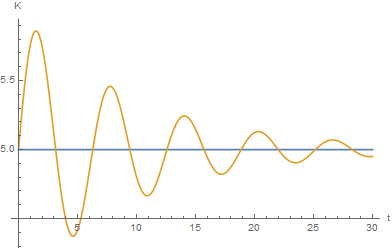
\includegraphics[scale = 0.7]{Thermostats/nose.png}
    \caption{K vs t in the NH algorithm. The blue line represents the value for the objective (average) kinetic energy.}
    \label{Kvtnh}
\end{figure}

\par The $\gamma$ keeps correcting the kinetic energy until it reaches (if lucky) the objective value $\bar{K}$. The rate at which the system reaches equilibrium is controlled by the mass of the thermostat ($M$) as well as the frequency of these damped oscillations. Choosing the parameter is not trivial at all. If we make $M$ smaller it will oscillate more frequently but this doesn't ensures a quicker relaxation.
\par These oscillations are one of the main problems with the NH algorithm, is very bad for relaxing the system. 
Normally, one should ensure the equilibrium of the system (with the Berendsen thermostat for instance) and once it reaches equilibrium one can simulate the production using the NH thermostat, that will give you the correct fluctuations. 

\par The other main problem is ergodicity. It's very easy to find a system which is non-ergodic using this algorithm: the harmonic oscillator. The phase space of the system may look like the figure (\ref{psnh}), where the possible positions doesn't form an ellipse as we should expect; instead the points sample across specific strips and there are regions left empty thus broken ergodicity: the resulting trajectory is dependent on our starting point. As solids (at least at low temperature) are simulated with harmonic oscillators then using the NH algorithm for this kind of systems is a bad practice. 

\begin{figure}[h!]
    \centering
    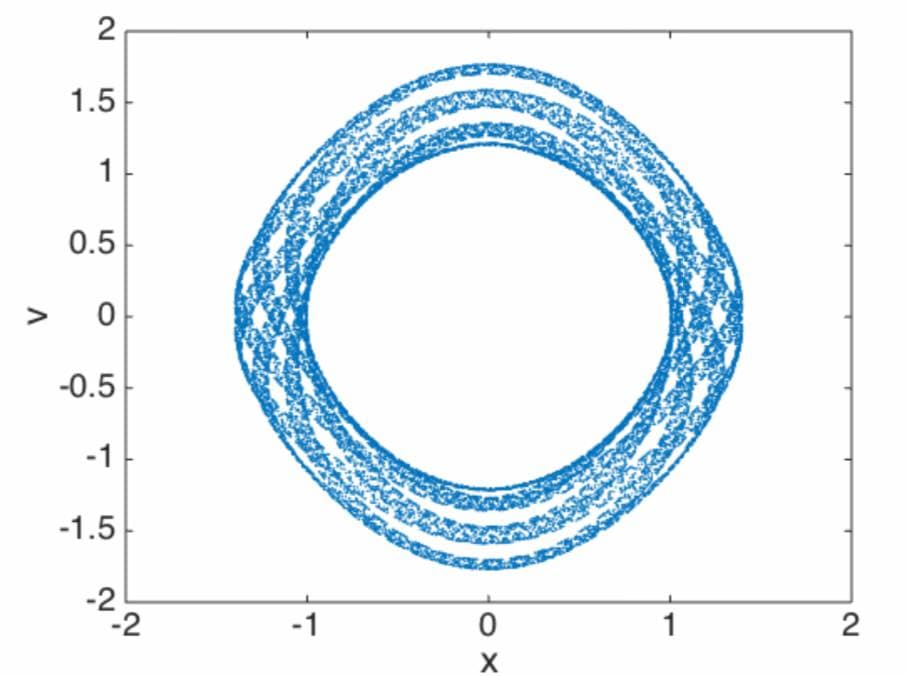
\includegraphics[scale = 0.5]{Thermostats/psnh.jpg}
    \caption{Phase space using the NH algorithm. Clearly non-ergodic.}
    \label{psnh}
\end{figure}


\par Nevertheless, there are several extended NH algorithms that correct this problem of non-ergodicity. Here, we mention three of them.

\subsubsection{5.2.7.1 Nosé-Hoover Chain}
Back in equation (\ref{ansatznh}) we can re-interpret the term $M \gamma^2/2$ as a kinetic energy, specifically, the kinetic energy of the thermostat. Having a new kinetic energy with a velocity $\gamma$, then we can add a thermostat for it, yielding in a \textit{thermostat for the thermostat}. We can iterate this process as much as we want, defining what we call \textit{Nosé-Hoover chain}:

\begin{equation}
    \begin{cases}
    dK = -2\gamma Kdt\\
    d\gamma_1 = \frac{2}{M_1}(K -\bar{K})dt - \gamma_1 \gamma_2 dt\\
    d\gamma_2 = \frac{2}{M_2}\left(\frac{\gamma_1 ^2 M_1}{2} - \frac{1}{2}k_B T\right)
    \end{cases}
\end{equation}

This solves the ergodicity problem at the price of making the system of equations more complicated. Since the chain reduces higher order fluctuations (as we now have a new thermostat that regulates the energy of the first one) then the system reaches equilibrium easier and as we keep adding terms the corrections tend to minimize fluctuations until we have an approximately constant energy thus defining the manifold (the ellipse for two dimensions) in the phase space. The typical number of $\gamma$ to reach a good value of ergodicity is four ($\gamma_1, \gamma_2, \gamma_3 and \gamma_4$).  
This process can be shown to be compatible with stochastic velocity re-scaling since a random number generator can arise after adding a very high number of terms in the chain.

\subsubsection{5.2.7.2 Nosè-Hoover-Langevin}
The idea is to use as a first element Nosè-Hoover thermostat, but as second element a Langevin thermostat:
\begin{equation*}
    \begin{cases}
    dK = -2\gamma Kdt\\
    d\gamma = \frac{2}{M}(K-\bar{K})dt - \color{blue}{\gamma \bar{\gamma}dt + \sqrt{2k_B TM\bar{\gamma}}d w}
    \end{cases}
\end{equation*} 
The \textcolor{blue}{blue} is the part substituting the second Nosè-Hoover thermostat. We added a friction $\bar{\gamma}$ and the corresponding noise, such that $\gamma$ samples from the correct distribution \ref{ansatznh}. This is yet another way to make the Nosè-Hoover ergodic.


\subsubsection{5.2.7.3 \textit{Massive} Nosé-Hoover Thermostat}
In this case, we assign a $\gamma$ for each degree of freedom of the system. In the original NHT there's only one $\gamma$ for the entire system, but in this case we will add a $\gamma$ for each of the $3N$ components for the velocity in the phase space. As we have a thermostat for each degree of freedom of the system we can consider this as a \textbf{local thermostat}. Furthermore, we can implement this massive NHT in a NH chain, so we have a chain of thermostat in every degree of freedom (so $12N$ $\gamma$ for our typical values). 
This massive NHT is common in ab initio simulations, e.g. in chemical reactions we'll have electron transfer then a lot of energy leaves/enters the system suddenly then we use a massive thermostat for the system to reach equilibrium quickly. 

